\chapter{Návrh systému a Implementácia}
Pri návrhu a implementácii našej aplikácie sme brali do úvahy výhody a obmedzenia systému \textit{IMS4} (\textit{Integrated Monitoring System}), ktorý je vyvíjaný spoločnosťou \textit{MicroStep-MIS s.r.o.}. Dôvodom je, že náš verifikačný systém bol navrhovaný ako prídavný modul pre IMS4.

V tejto kapitole stručne zhrnieme návrh systému a opíšeme kľúčové časti implementácie.


\section{Návrh systému}
Našu aplikáciu sme sa snažili navrhnúť jednak ako samostatný produkt schopný extrakcie a spracovania meteorologických dát a výpočtu verifikačných štatistík, ale taktiež aj ako súčasť systému IMS4. Toto sme dosiahli tak, že sme rozdelili systém na 2 balíky: \textit{verifikačný} a \textit{vizualizačný}. Na obrázku \ref{fig:system} môžme vidieť schematický návrh systému.

\textit{Verifikačný balík} tvorí jadro celého systému a zohráva viacero úloh. V prvom rade je jeho úlohou extrakcia dát z rôznych dátových zdrojov do tabuliek predpovedí a pozorovaní. Tieto tabuľky sa následne predspracúvajú (párovanie, konverzia fyzikálnych jednotiek, filtrovanie, identifikácia chýbajúcich dát...) a posúvajú sa do časti na výpočet štatistík. Na základe konfigurácie sa spočítajú rôzne štatistiky, ktorých výsledok je výstup z tohoto balíka.

\textit{Vizualizačný balík} chápeme ako vymeniteľnú časť systému. Vďaka tomuto môže byť vizualizácia v podobe interaktívnej obrazovky, ktorá je súčasťou systému IMS4, ale taktiež generovaná automaticky do statických obrázkov na disku.

\begin{figure}
	\centering
	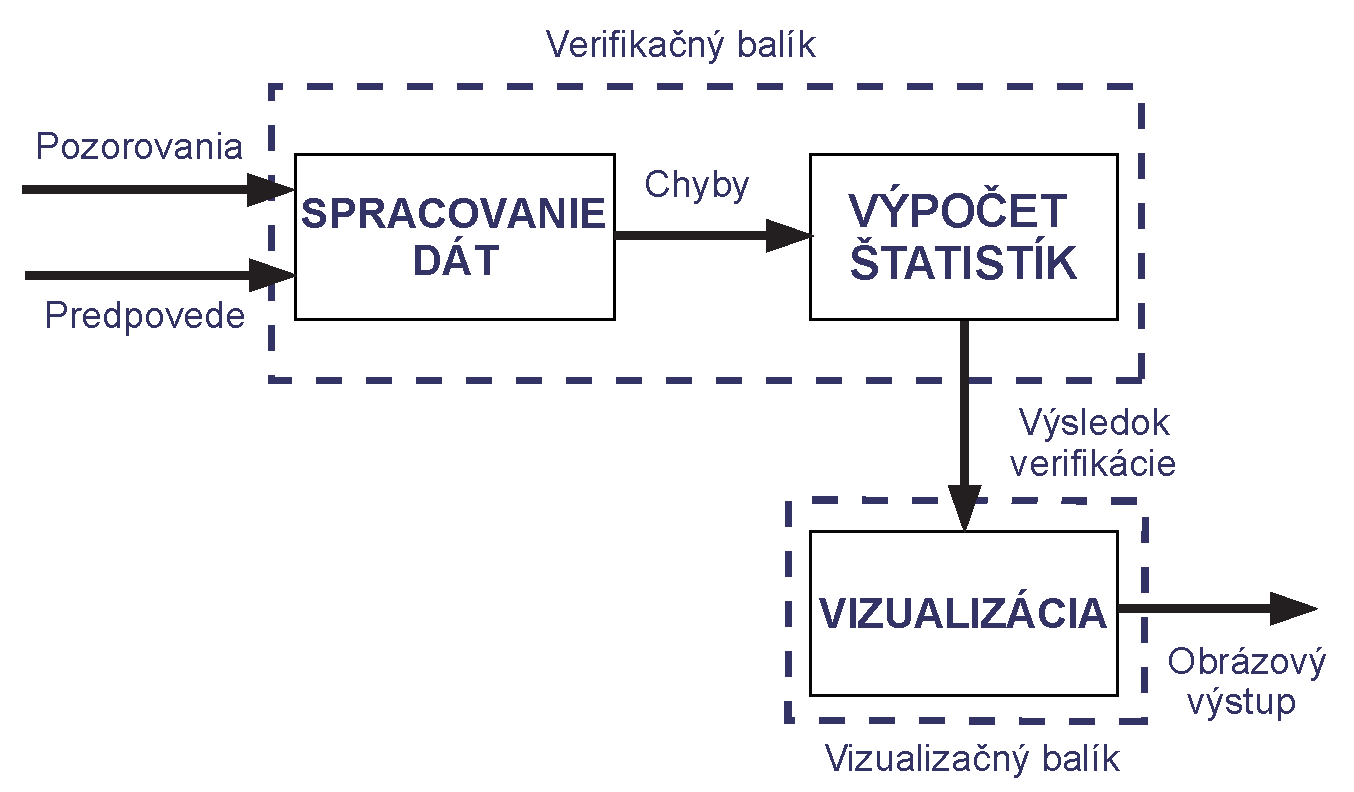
\includegraphics[width = 4.5in]{system}
	\caption{Schematický popis systému.}
	\label{fig:system} 
\end{figure}

Ak by sme mali systém opísať v pojmoch vizualizácie informácií, tak tieto dva balíky rozdeľujú vizualizačnú \textit{pipeline} na dve časti (Pozri obrázok \ref{fig:pipeline}). Verifikačný balík sa stará o analýzu dát pomocou predspracovania a matematického modelu verifikačných štatistík a taktiež sa stará o filtrovanie dát. Zvyčajne filtrovanie prebieha na základe interakcie užívateľa. V našom prípade sme však uvažovali aj o možnosti, že vizualizácia nebude interaktívna, preto sme filtrovanie umiestnili do verifikačného balíka a vykonáva sa na základe konfigurácie systému. 

Filtrované dáta putujú do vizualizačného balíka. V ňom sa vykonáva zobrazenie hodnôt na vizuálne parametre jednotlivých prvkov vizualizácie, tak ako sme to opísali v kapitole \ref{chap:design} \textit{Návrh vizualizácie}. Takéto dáta sa následne vykreslia do obrázka alebo na obrazovku, čím sa ukončí vizualizačná pipeline.


\begin{figure}
	\centering
	\includegraphics[width = 6in]{pipeline}
	\caption{Rozdelenie prvkov vizualizačnej pipeline do verifikačného a vizualizačného balíka. Obrázok pipeline pochádza zo stránky \protect\url{http://www.infovis-wiki.net}.}
	\label{fig:pipeline} 
\end{figure}

\section{Použité technológie}
V tejto časti rozoberáme technológie použité pre implementácii systému a uvádzame dôvody ich použitia.

\subsection{Java}
Primárnu časť systému - \textit{verifikačný balík} sme implementovali v jazyku \textit{Java}, konkrétne vo verzii 1.5. Toto je prvé obmedzenie, ktoré na nás kladie systém IMS4, keďže použitie vyššej verzie (momentálne je dostupná už verzia 1.8) by spôsoboval problém s kompatibilitou.

Java ako programovací jazyk je veľmi rozšírený a obľúbený, vďaka čomu je dostupných pomerne veľké množstvo knižníc, nevynímajúc originálne knižnice zahrnuté v systéme IMS4. Tieto knižnice sme využili pri implementácii aj my. Môžme spomenúť 3 knižnice, z ktorých sú dve interné a jedna pôvodne externá s pridanou funkcionalitou. Prvé dve spomenuté sú \textit{Log} - používaná na logovanie a \textit{X2O}, ktorá sa používa na mapovanie javovských objektov na XML štruktúru a späť pomocou \textit{Java Reflection API}. My sme X2O použili pri ukladaní a načítavaní konfiguračných súborov. Posledná knižnica je NetCDF a pochádza od americkej organizácie \textit{Unidata}, ktorú zastrešuje \textit{UCAR}. Jedná sa o opensource produkt na čítanie dát zo súborov vo formáte GRIB. My využívame upravenú verziu NetCDF grib-6.0 obzvlášť kvôli Jave 1.5, aj keď sú dostupné novšie verzie \footnote{Najnovšia je NetCDF-Java-4.5, ktorá zoskupuje všetky ďalšie podobné produkty od Unidata.}.

\subsection{JavaScript}
Systém IMS4 využíva webové stránky na vytváranie GUI. Z tohto dôvodu sme sa rozhodli, že vizualizáciu budeme produkovať priamo v prehliadači pomocou \textit{JavaScriptu}. Podovbe ako Java, aj JavaScript je veľmi populárny a preto vzniklo veľké množstvo rôznych knižníc, medzi ktorými sú aj mnohé vizualizačné.

\subsubsection{D3.js}
D3 (\textit{Data Driven Documents}) sme zvolili ...


\section{Extrakcia a spracovanie dát}

\subsection{CSV}

\subsection{Webové zdroje}

\subsection{GRIB}

\subsection{...}

\section{Konfigurácia systému}


\section{Obrazovka vizualizácie}